%%
\chapter{Domain modeling and goal definition in EMF and \viatra{}}
%%



Domain modeling is an essential part of our framework, as models are the main artifacts which from the monitoring code will be generated.
The initial artifacts are the EMF (Eclipse Modeling Framework) based metamodel and the monitoring queries as \viatra{} graph patterns.

\section{Eclipse Modeling Framework}


\begin{figure}[h]
	\begin{center}
		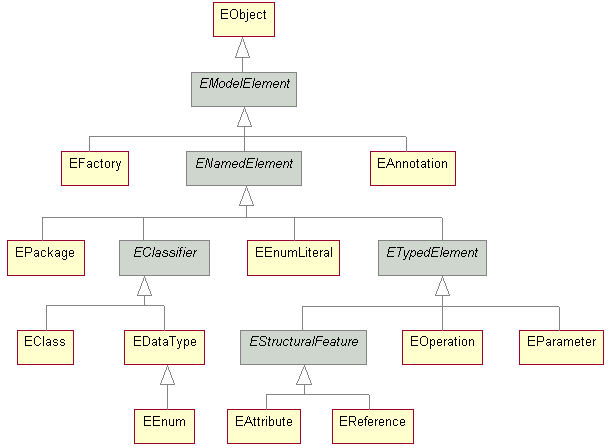
\includegraphics[width=0.5\textwidth]{figures/EcoreHierarchy.png}
		\caption{Hierarchy of Ecore elements}
		\label{fig:ecore-model1}
	\end{center}
\end{figure}

\begin{figure}[h]
	\begin{center}
		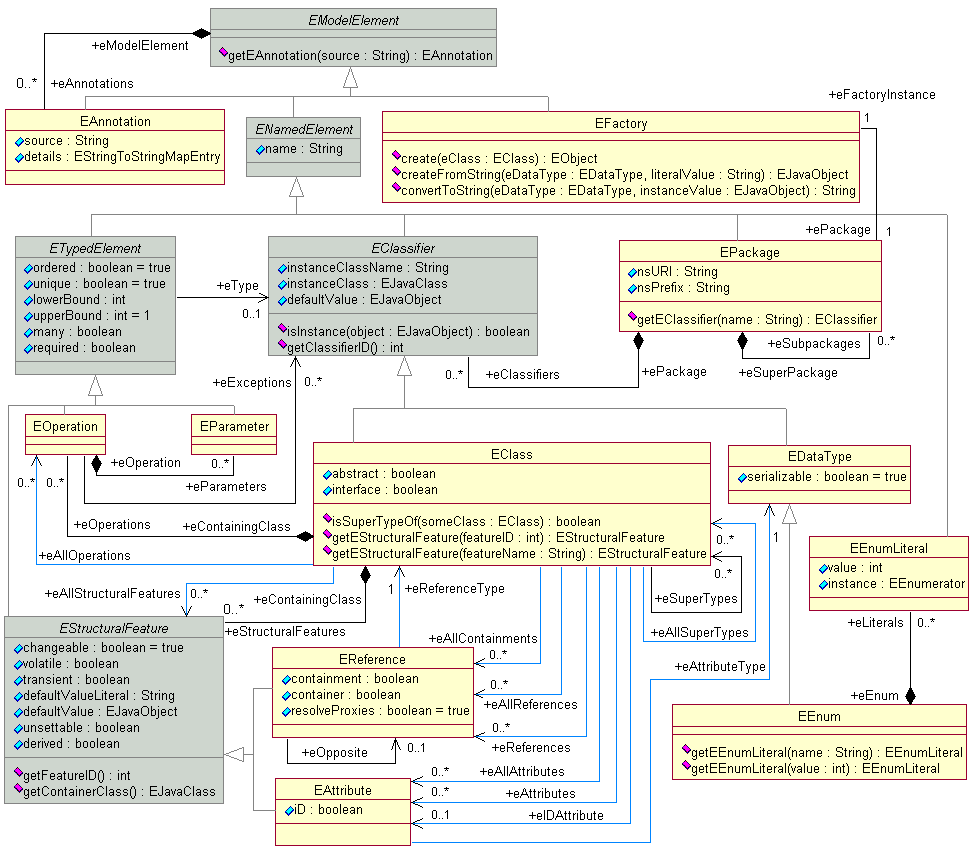
\includegraphics[width=\textwidth]{figures/EcoreRelations.png}
		\caption{Relations between Ecore elements}
		\label{fig:ecore-model2}
	\end{center}
\end{figure}
			